
\section{The RegionSeeker Framework}
\label{sec:rs}

The RegionSeeker framework is an automated methodology that 
identifies candidates for HW acceleration from application source 
code. An extensive SW analysis, based on the LLVM compiler infrastructure,
performs, apart from
the identification, an estimation of the performance gain, along with
the HW resources cost, of each candidate. Subsequently given a HW resources
constraint, a selection of the identified HW accelerators takes place that
maximizes the cumulative performance gain.
In the following subsections the methodology is presented in detail, as well as
experimental results from the CHStone benchmark \cite{HaraMay08} suite.

\subsection{Methodology}
\label{subsec:meth}

There are three parts comprising the methodology, detailed as follows.
The first step is to automatically identify valid regions that are suitable candidates
for HW acceleration. Secondly, an estimation of their potential merit, in terms of cycles saved
(the difference between SW and HW execution cycles),
is computed along with the respective cost, which is the HW resources (area) required
for each region. Finally, a selection algorithm is utilized in order to optimally solve the 
problem of selecting a subset of these
regions that maximize the accumulated merit under a given cost, i.e., an area constraint.

\subsubsection{Region Identification}
\label{subsec:reg_id}

To identify regions in both an automatic and efficient way, a
 \emph{Region Identification} pass was developed under the version 3.8 
of the \emph{LLVM Compiler framework} \cite{LattnerMar04}. 
The pass receives as input applications developed in C or C++ and performs 
their analysis at the Intermediate Representation (IR) level, a type
of code used internally by LLVM to represent source code and allow
data flow analysis and optimizations.\par

The pass iterates over every function of an
 application and, using the existing \emph{RegionInfo} LLVM pass 
\cite{GrosserApr12}, identifies regions within every function.
%, as seen in Figure \ref{fig:region}. 
Subsequently, nodes that cannot be synthesized, such as system
calls or calls to functions that are not inlined, are identified 
and labeled as forbidden.
%forbidden nodes inside regions are identified and labeled, such as system
%calls or calls to functions that are not inlined. 
The regions containing
these nodes are marked as invalid. Conversely, the valid regions are 
evaluated by a profiling-via-instrumentation routine.
Profiling via
instrumentation requires generating an instrumented version of the
code, which gives more detailed results than a sampling
profiler. 
The output of the profiling is a file that contains information regarding 
the execution frequency of each basic block and the total number of calls to each 
function, i.e., the execution frequency of each function.
Using this information, the basic blocks are annotated
 in each function with their respective execution frequency. 
% with the aid of \emph{ClrFreqCFGPrinter} LLVM pass \cite{ZacharopoulosMar17},
 %that I have developed.


% LLVM RegionSeeker Analysis Pass.
% %
\begin{algorithm}[t]
\begin{flushleft}
\textbf{Input:}  Application written in C/C++\\
\textbf{Output:} List of Identified and Profiled Regions\\
\end{flushleft}
\begin{algorithmic}[1]
\Function{$RunOnFunction()$}{}
\State\Call{$Region\_List=NULL$}{}
\State\Call{$RI=getRegionInfoAnalysis()$}{}
  \For {$Region\ in\ Function$}
    \If {\Call{$RegionIsValid()$}{}}
      \State\Call{$EvaluateRegion$}{Region}
      \State{$Region\_List.Add(Region)$}     
    \EndIf
  \EndFor
  \State{$return\ Region\_List$}  
\EndFunction

\State
\State{$/* Estimate\ Merit\ for\ Region*/$}
\Function{$EvaluateRegion$}{Region}
  \For {$Basic\ Block\ in\ Region$}
    \State\Call{$getProfilingInfo$}{Basic\ Block}
  \EndFor
\EndFunction
\end{algorithmic}
\caption{LLVM Analysis Pass - Region Identification} 
\label{algo:reg}
\end{algorithm}

\subsubsection{Merit and Cost Estimation}
\label{subsec:mer_cost}

The Region Identification pass, apart from the identification of regions detailed above, 
performs an early evaluation of the merit and cost of a region, implemented
directly within the LLVM tool-chain. The evaluation relies on the LLVM intermediate
representation and does not need any manual modification to perform function out-lining
on the benchmark source code. 
The estimation of merit and the cost of a region is performed as follows.\par

\emph{Merit Estimation.} 
The merit of a region is defined as the total number of cycles saved in a HW accelerator 
implementation compared to the respective SW implementation of the same piece of runtime 
of a given application. Therefore the merit of a HW accelerator is estimated as the 
difference between the \HW\ and \SW\ run time, across all its invocations in an application,
taking into account the invocation overhead of calling a HW accelerator in a specific 
heterogeneous architecture. The estimation of the HW run time is computed first in the 
basic block (BB) level as the the critical path of the latency (in clock cycles) of the Data 
Flow Graph (DFG) nodes. Runtime profiling information is used in order to determine the execution 
frequency of each BB.
Subsequently the delay of the entire region in HW is estimated by multiplying the critical path
delay of each BB with the respective execution frequency and finally summing up the products, 
according to the specific BBs that comprise the region.
Software run-times are estimated in a similar fashion, but instead of computing critical paths 
at the BB level, the sum of the latency (in clock cycles) of all its constituent operations is 
computed, modeling that these are processed sequentially in software.\par

\emph{Cost Estimation.} On the other side of the evaluation, the cost of a region 
is estimated as the area (or HW resources) required to implement its DFG nodes. The area 
is computed as the sum of look-up tables that is required for
the DFG nodes of the respective HW accelerator. Each DFG node may take up a different amount
of loop-up tables according to its complexity. The characterization for each DFG node was carried
out with the aid of Vivado, a commercial \HLS\ tool, targeting a Virtex7 FPGA.\par
% and its merit as the cycles saved between SW
% and HW execution, where the latter is the delay of the nodes on the
% DFG critical paths. Runtime profiling information is used in both SW and
% HW latency estimations in order to determine the number of invocations for
% each candidate.\par
The final output of the analysis pass is a list of valid regions, 
or else accelerator candidates, each annotated with an estimated merit and cost.
The region list output is in turn processed by the 
\exact\ selection algorithm implemented as standalone program in C++.
% selection algorithms exact and greedy implemented as standalone programs in C++.


\subsubsection{Region Selection Algorithm}
\label{subsec:sel_algo}

Given a merit $M()$ and cost $C()$ function for each region 
we can formulate the problem of selecting accelerators as follows:\\
\textbf{Problem: Region Selection}
Let $\mathcal{R} = \{ R_1, R_2, \ldots, R_n \}$ be a set of regions,
with associated cost and merit functions $C$ and $M$.
For any subset $X\subseteq \{1,2,\ldots,n\}$ of regions,
we denote by $M(X) = \sum_{i\in X} M(R_i)$ the sum of the merits of
its regions, and we denote by $C(X) = \sum_{i\in X} C(R_i)$ the sum of
the costs of its regions.

We want to select a subset $X$ of regions such that
\begin{enumerate}
\item No two regions belonging to the same CFG overlap, i.e.,
  $V(R_i)\cap V(R_j) = \emptyset$, for all $1\le i,j\le n$
\item The cost $C(X)$ is within a user-given cost budget $C_{\max}$
\item The merit $M(X)$ is maximized
\end{enumerate}


This problem definition maps to what we have identified in
Section~\ref{sec:mot} as the designer aim: given an available
accelerator area, extract as much as possible of the computation,
under the constraint to require no more than that area, in order to
maximize the resulting speedup.\par

\begin{figure*}[t]
\centering
%\includegraphics[width= \linewidth]{figs/figs_from_pptx/exact_tree.pdf}
\includegraphics[width= .9 \linewidth]{Figs/exact_tree.pdf}
\caption{Tree exploration performed by \exact, for the running example
  of Figure~\ref{fig:cfg-example}, and for a cost budget of 35.}
\label{fig:exact_tree}
\end{figure*}

An exponential, \exact\ branch-and-bound method
based on a binary-tree search was derived in order to solve optimally 
the Region Selection problem. The algorithm converges to an
% is implemented so that it finds the 
independent set of regions that maximizes merit under 
a given cost.
This process can be exemplified through
 Figure~\ref{fig:exact_tree}: given an initial set $P$, that includes all
 valid regions identified, and a set $X$, that is initially an empty set and 
is going to be the subset of $P$ that maximizes merit under a given cost.
The root of the tree represents the empty set, and set $P$ at this
point contains all regions. Furthermore an overlapping graph among regions 
shows whether there is overlapping among valid regions contained in $P$, 
such that it poses the restriction of not allowing the selection of regions 
that overlap with each other, i.e., containing at least one BB that is common. 
The overlapping graph is seen as well in Figure~\ref{fig:exact_tree}.
As the algorithm starts the exploration, inclusion of region A is first
considered, and the set P is updated by removing all regions overlapping
with A: $P = \{E\}$. According to the merit and costs of all regions
in this example, shown in the table within the picture, the merit (60)
and cost (35) of the solution currently explored is also updated.\par

At every point of the exploration, a new node $u$ is considered for
addition in the current independent set.
If there is no node $u$
satisfying condition $2$ of the Region Selection Problem, the algorithm
records the set $X$ and backtracks, as $X$ is maximal with respect to
condition $2$.  For the running example in
Figure~\ref{fig:exact_tree}, the cost budget $C_{\max}$ is equal to
$35$. Hence, exploration stops at $X=\{A\}$ because the cost budget
has been reached, and backtracks. The next region chosen is $B$, sets
$X$ and $P$ are again updated accordingly, to $X=\{B\}$ and
$P=\{C,D,E\}$, and exploration continues until the selection algorithm
converges.\par

Two optimizations are implemented in the exact selection algorithm in order 
to avoid unnecessary exploration. Optimization 1 performs a look up in order 
to determine whether the maximum recorded merit can be reached by the 
regions contained in $P$ or not. If not the exploration stops and backtracks.
Optimization 2 ranks the valid regions in terms of merit so that the first 
region considered for inclusion in $X$ is the one with the maximum merit.



\begin{figure}[h!]
\centering
\hspace*{-1cm}
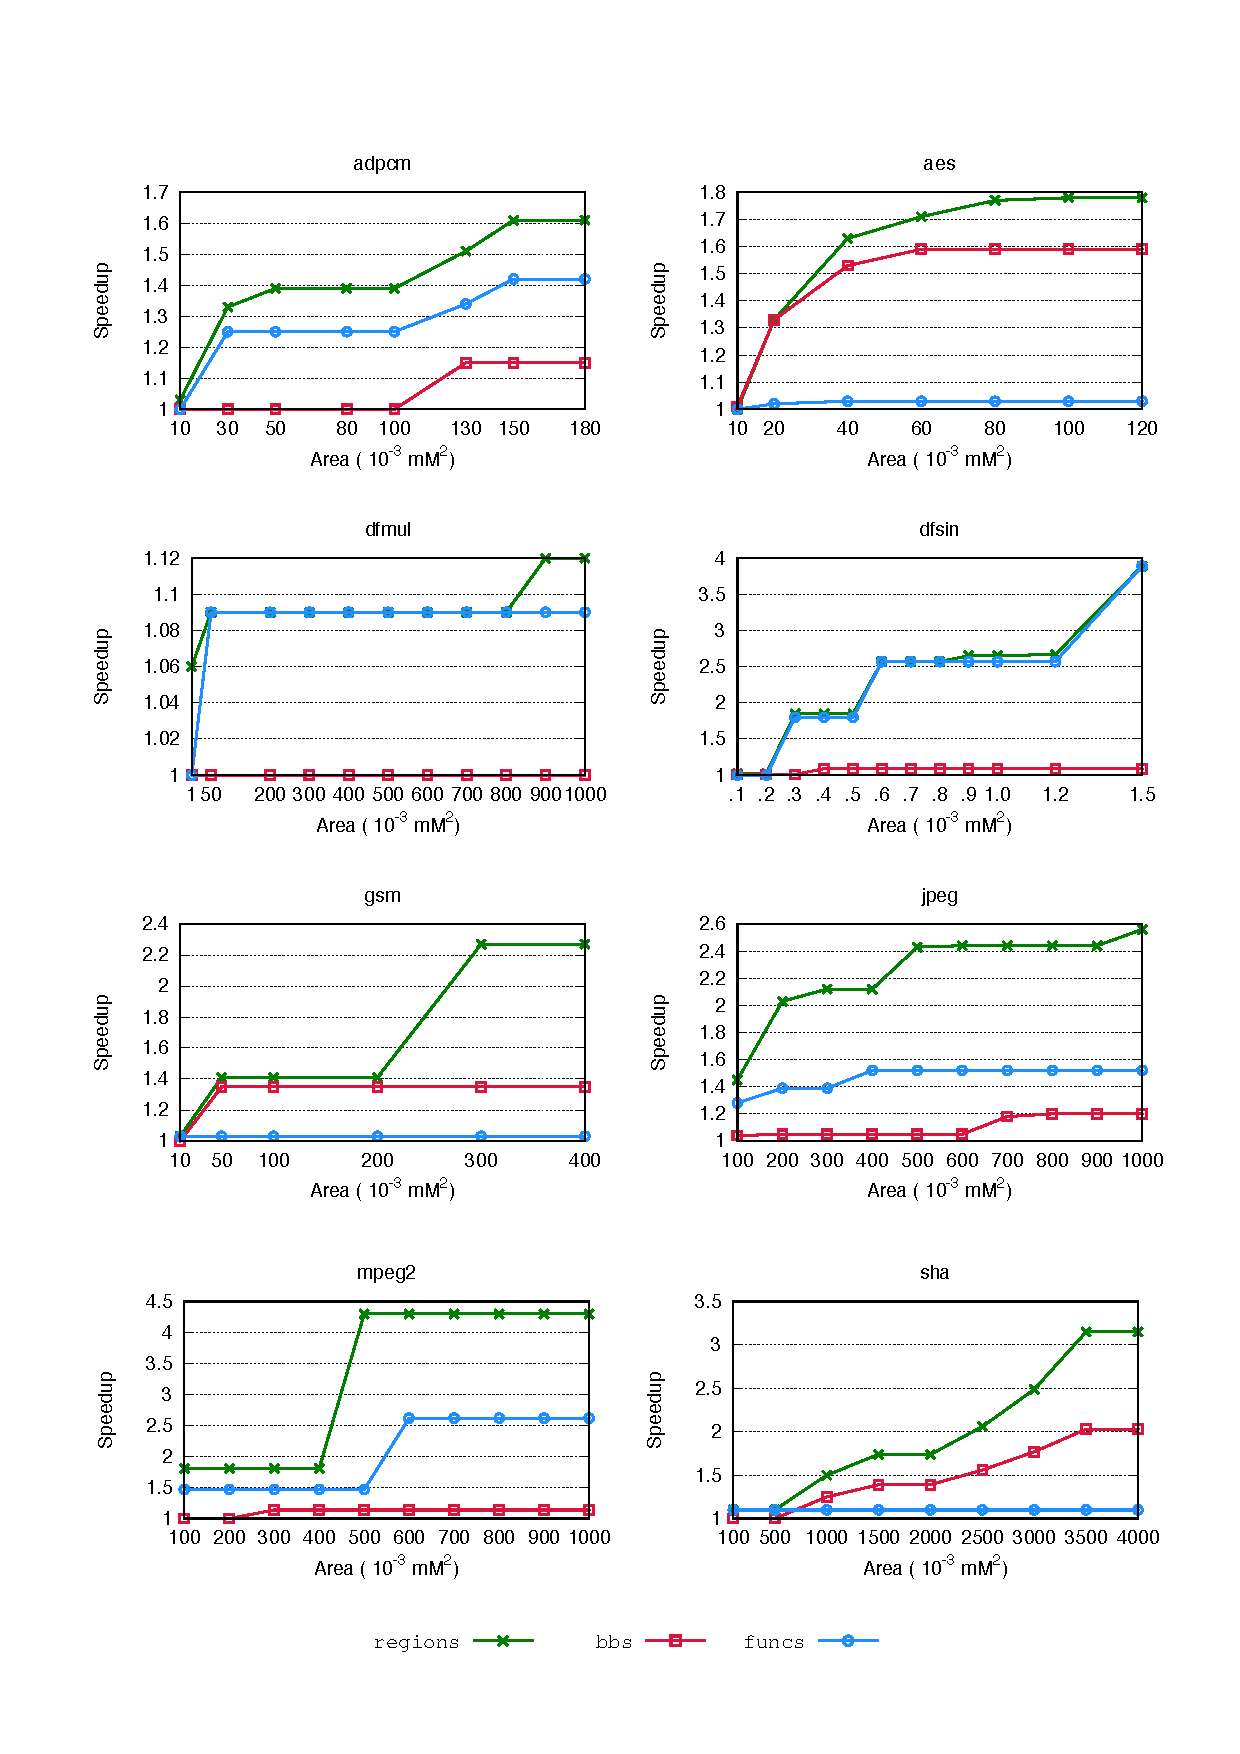
\includegraphics[width= 1.1 \linewidth]{figs/regions_aladdin}
\caption{Comparison of speedups obtained on eight CHStone benchmarks
  by selecting regions, only basic blocks and only functions, varying
  the area constraint, using Aladdin and Gem5 for Speedup and Area evaluation.}
\label{fig:regions_aladdin}
\end{figure}

\subsection{Experimental Results}
\label{subsec:exp}

The evaluation of the \rseeker\ framework took place by assuming a system constituting a single 
SW processor and multiple HW accelerators, exchanging shared data with \plms. The processor 
activates the accelerators via a memory-mapped interface, thus requiring a transaction on the 
system bus. When activated, accelerators read and write data to and from the \plms, computing 
their outputs, which can then be accessed by the processor. Accelerators are interfaced to \plms\ 
with ports having a latency of one clock cycle. The control interface between the processor and 
the accelerators was modeled with a latency of 10 clock cycles.\par

The run-times of the non-accelerated SW part of the considered
benchmarks were measured using the Gem5
simulator~\cite{BinkertFeb11}, modeling an ARMv8-A processor with an
issue width of 1. The processor model is atomic, with in-order
execution. It is interfaced with separate instruction and data
memories with an access latency of one clock cycle.\par

Hardware execution times were retrieved using two different HLS 
frameworks: the Aladdin simulator and the Xilinx Vivado HLS
commercial tool-suite.  Aladdin targets ASIC implementations.  It
provides a fast evaluation, but does not produce a synthesizable netlist
as output; nonetheless, the estimations offered by this tool are
within 1\% of the ones derived from an RTL implementation
\cite{ShaoJul14}.  Hardware instances generated with Vivado HLS are
instead intended for FPGA designs. Synthesis-runs within this
framework are more time-consuming, but provide exact area (HW resources
in terms of Look Up Tables and Flip Flops)
and latency (number of cycles) values of each accelerator, as well as a direct
path to its realization.  In both cases, default implementations of
the accelerators were considered, i.e., no optimizations were applied to the
implemented HW accelerators.\par

The benchmarks that were used during the experimental phase are embedded applications
of varying size from the CHStone benchmark suite \cite{HaraMay08}.
\adpcm\ performs an encoding routine and \aes\ is a symmetric-key encryption algorithm. 
\dfmul\ and \dfsin\ are small kernels that perform double-precision 
floating-point multiplication and sine functions employing integer arithmetics. 
\gsm\ performs a linear predictive coding analysis, used in mobile communication. 
\jpeg\ and \mpeg\ are larger applications, implementing JPEG and MPEG-2 compression, respectively.
Finally, \sha\ is a secure hash encryption algorithm, used for 
the generation of digital signatures and the exchange of cryptographic keys.\par

% \begin{figure}[h!]
% \centering
% \hspace*{-1cm}
% 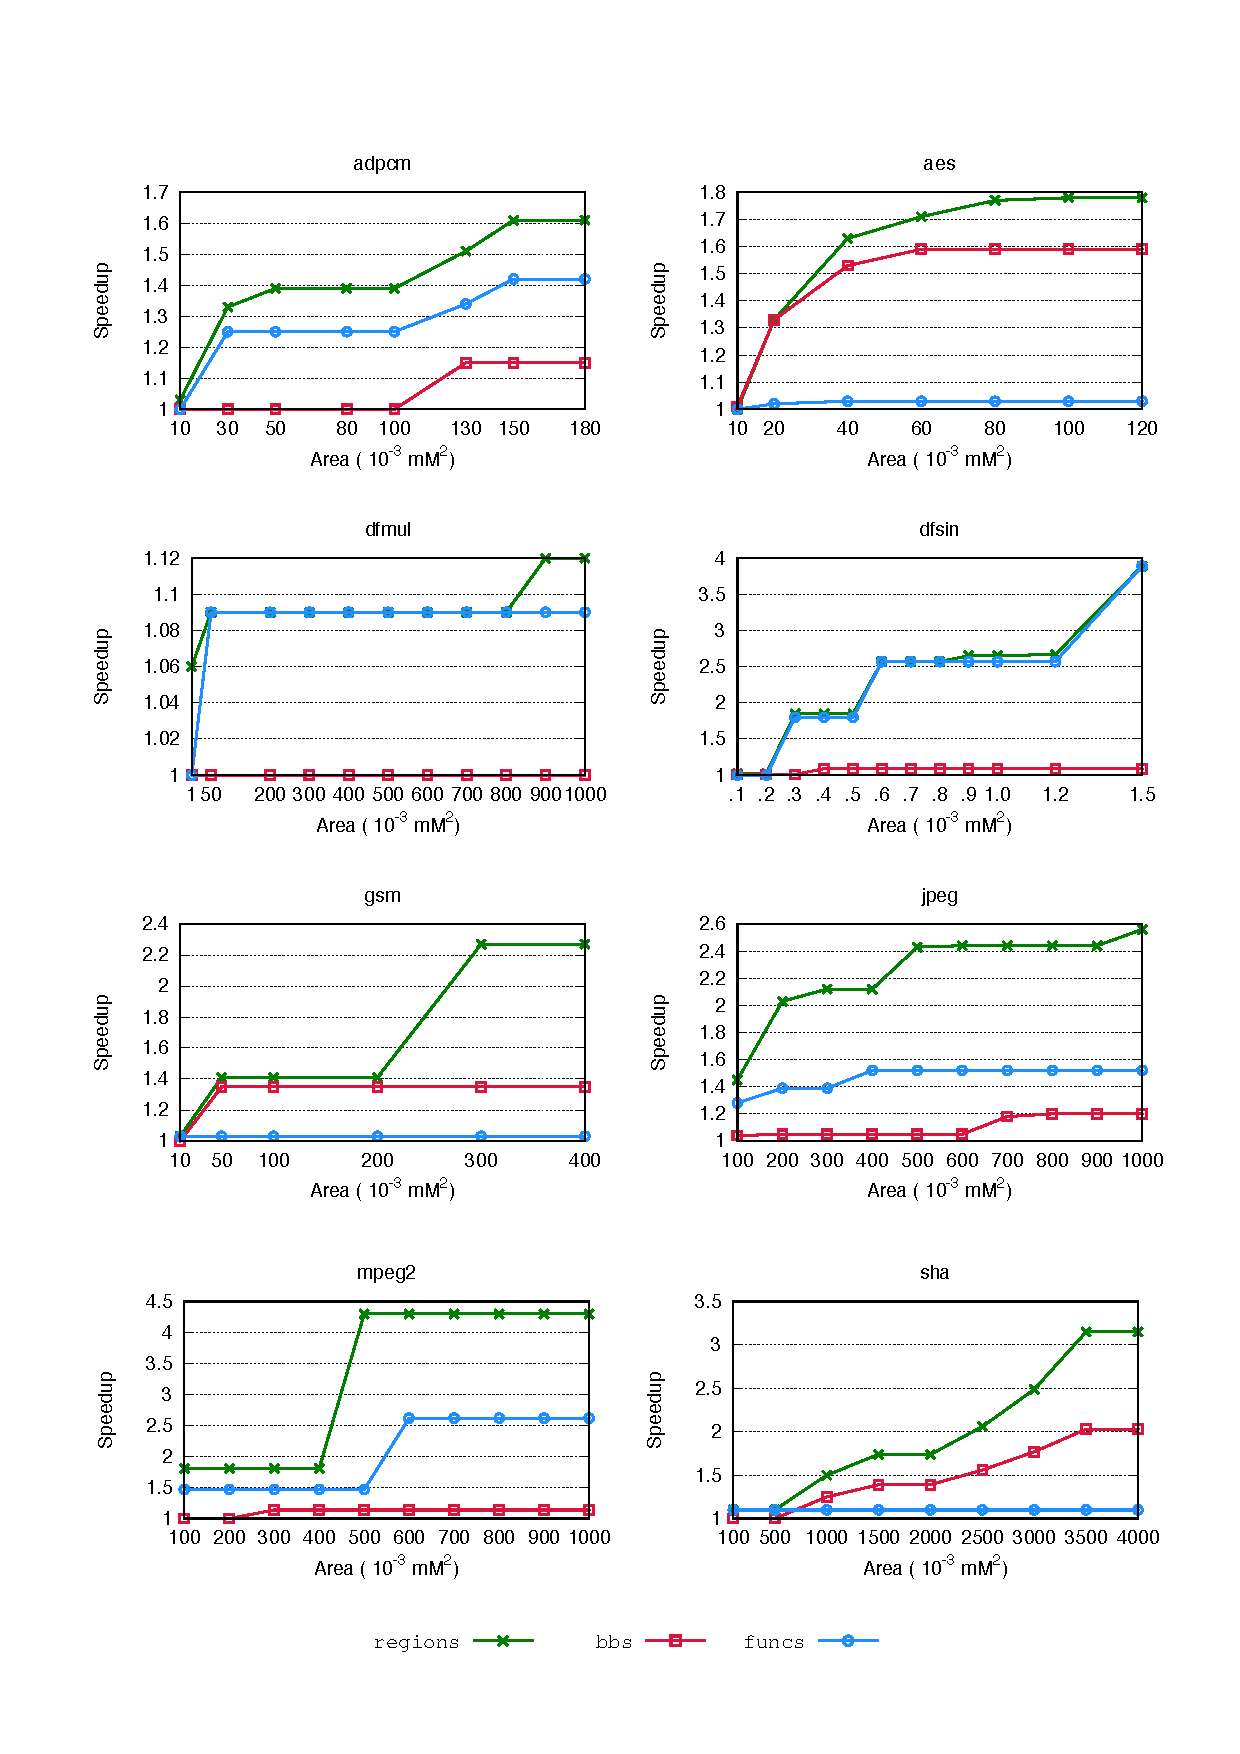
\includegraphics[width= 1.1 \linewidth]{figs/regions_aladdin}
% \caption{Comparison of speedups obtained on eight CHStone benchmarks
%   by selecting regions, only basic blocks and only functions, varying
%   the area constraint, using Aladdin and Gem5 for Speedup and Area evaluation.}
% \label{fig:regions_aladdin}
% \end{figure}

Figure~\ref{fig:regions_aladdin} showcases the achieved
speedup, when employing Aladdin, by the accelerators selected by
\rseeker\ (labeled \texttt{regions} in the figure), with respect to
the entire run-time of the applications and for different area
constraints.  For small-to-medium size applications such as \adpcm,
\aes, \gsm\ and \sha\ speedup gains for \rseeker\ vary from 1.6x up to
3.2x. For smaller kernels, larger variations can be observed, as for
\dfmul\ and \dfsin\ the speedup reaches 1.12x and 3.9x respectively.
Finally, for larger benchmarks such as \jpeg\ and \mpeg\, speedup is
fairly significant: 2.5x for the former and up to 4.3x for the latter
can be reached using \rseeker.\par

\begin{figure}[h!]
\centering
\hspace*{-1cm}
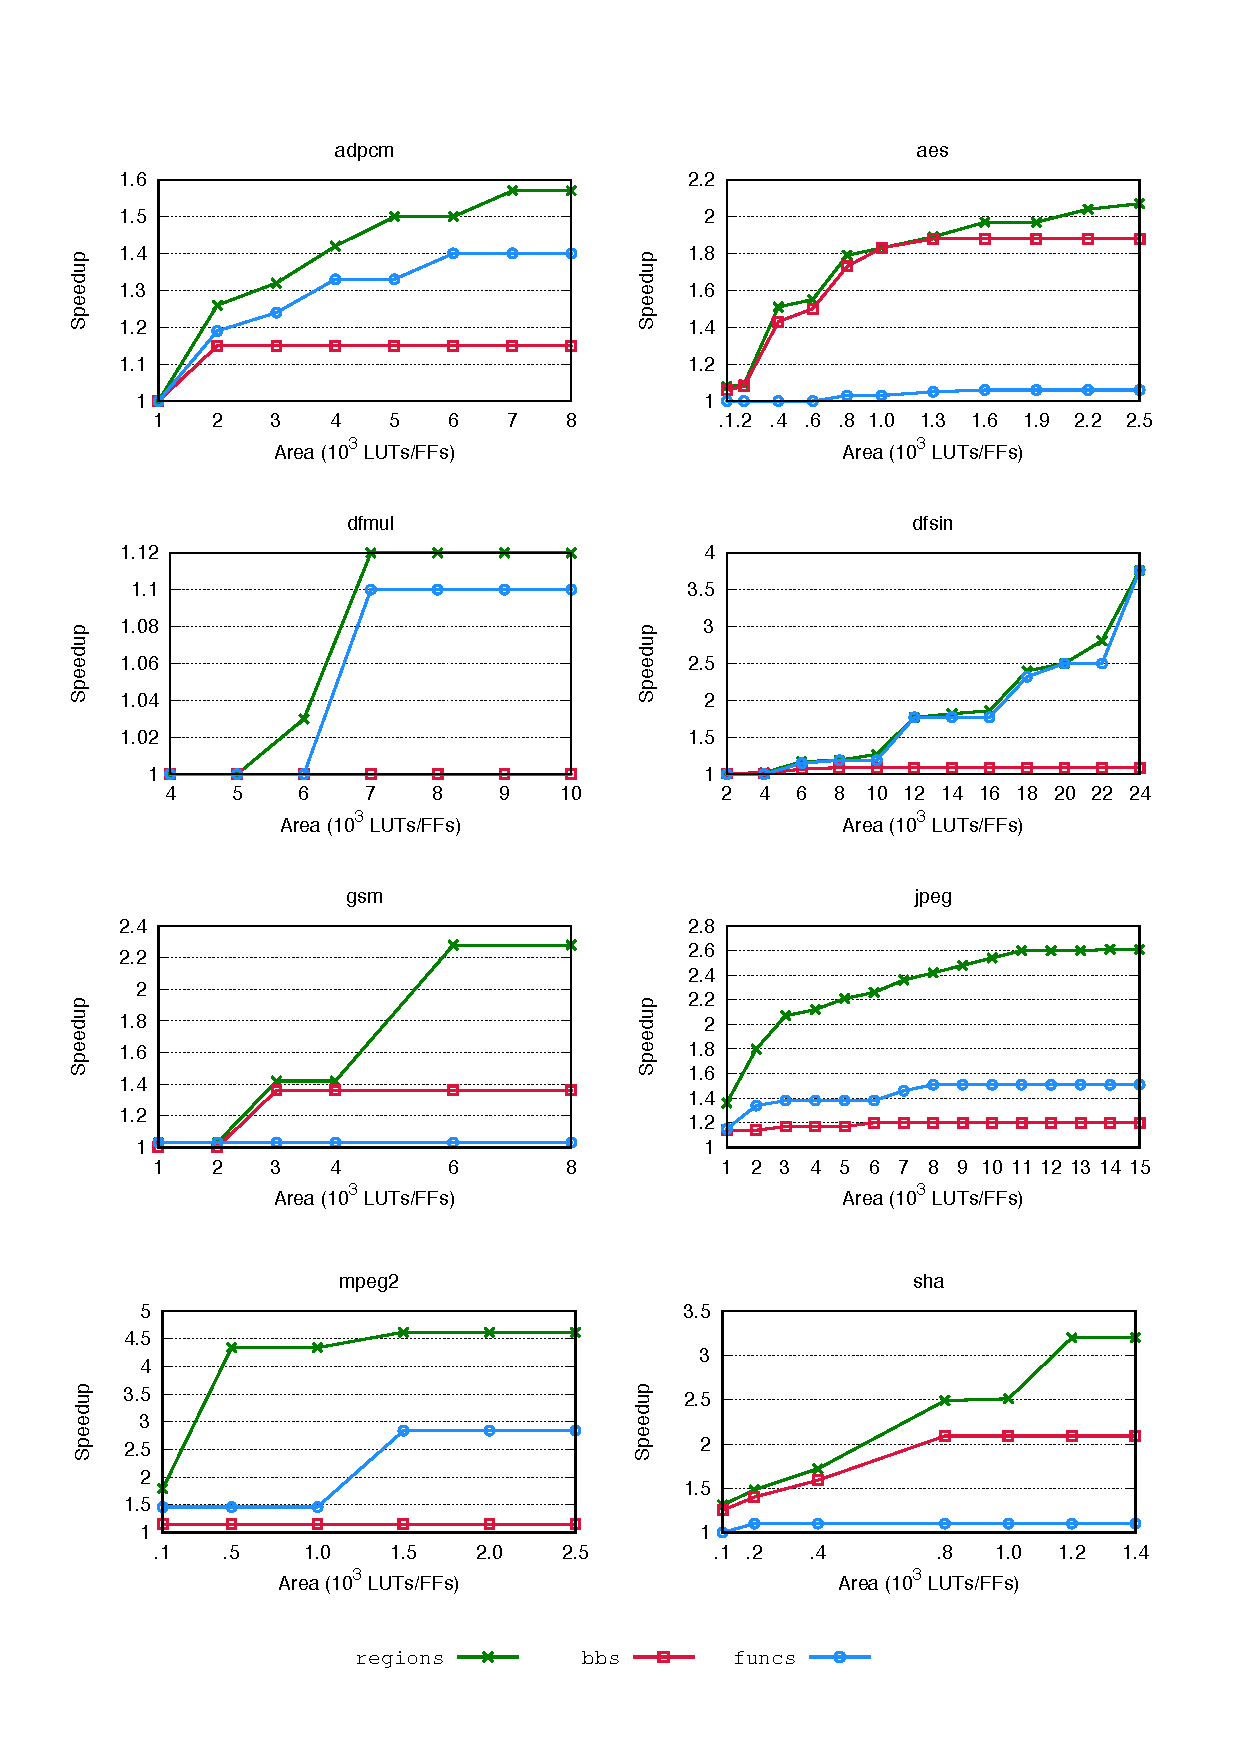
\includegraphics[width= 1.1 \linewidth]{figs/regions_vivado}
\caption{Comparison of speedups obtained on eight CHStone benchmarks
  by selecting regions, only basic blocks and only functions, varying
  the area constraint, using Vivado HLS and Gem5 for Speedup and Area evaluation.}
\label{fig:regions_vivado}
\end{figure}

Similar trends are observed when Vivado HLS is instead used for the
accelerator synthesis, as reported in
Figure~\ref{fig:regions_vivado}: \rseeker\ consistently outperforms
\SoTA\ approaches which target either single basic blocks or
entire functions, across all benchmarks. These results 
highlight that the achievable speedups
are highly influenced by which segments of applications are selected
for accelerations, and that such choice is only marginally influenced
by the adopted merit and cost estimation tool. In fact, this was verified 
across the two sets of experiments, as the regions chosen were
the same in 80\% of the cases. As an example, out of 10 regions
selected to achieve a 2.2x speedup for the \jpeg\ benchmark, 8 are the
same when using either Aladdin or Vivado HLS for merit and cost
estimation, and the ones that differ contribute to less than 14\% of
the provided gain.\par


\begin{figure}[h]
\centering
%\hspace*{-2cm}
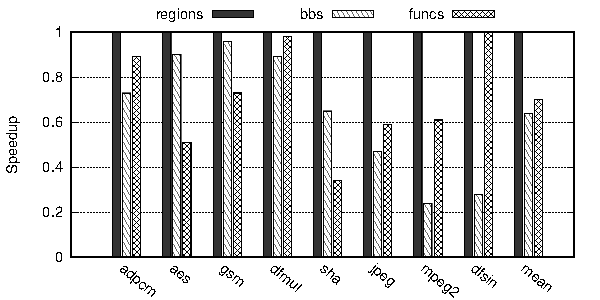
\includegraphics[width= 0.9 \linewidth]{figs/rbf_max_norm_all}
\caption{Normalized Speedup of RegionSeeker with respect to function and basic block selection, 
considering, for each benchmark, a fixed area constraint. Synthesis performed with Vivado HLS.}
\label{fig:regions_all}
\end{figure}

Finally, in Figure \ref{fig:regions_all} a summary of the performed experimental 
exploration is presented. It reports the normalized speedups
obtained by \rseeker\ compared to basic block and function
identification, when a fixed area budget is considered and
Vivado HLS are employed. The mean column illustrates that,
on average, \rseeker\ achieves approximately 30\% higher speedups
with respect to the two baseline methods. Moreover, while in some
cases the baselines match the performance of \rseeker\ (e.g.: \gsm\
for basic blocks, \dfsin\ for functions), neither of them can achieve that
consistently across applications, stressing the suitability of control-flow regions as
HW accelerator candidates.\par

The speedup that can be obtained by accelerating basic blocks is
hindered by their small granularity and, consequently, the high number
of HW accelerators invocations by the SW processor, i.e., the switches 
between software and hardware execution. Moreover, in this
setting many optimization opportunities
during the hardware implementation of the accelerators are missed,
because they only arise when control flow is considered, as is instead the case
for regions.\par

On the other hand, the speedup derived by selecting whole functions
trails the one corresponding to regions, because of two
reasons. First, function selection is limited to the ones which do not
present forbidden nodes, and this may rule out promising regions
within them. Second and more importantly, it is inflexible from
an area viewpoint, which is especially visible when few hardware
resources are available for acceleration. In those cases, the
selection of functions often detects only few feasible candidates,
with a small merit (e.g. in Figure \ref{fig:regions_aladdin}: \jpeg\ and 
\mpeg, for an area of less than 0.5 $mm^2$).\par

This limitation, though, is not present in regions, as simply the part
referring to individual hotspots inside a function can be available
for selection. Indeed, the performance of \rseeker\ stems from the high
flexibility of the selection approach, as it allows the consideration of
the entire spectrum of granularity ranging from whole functions to
single loops, ultimately enabling a better exploitation of speedup for
a given area budget.